  %
% LATEXBONES
%
\documentclass[a4paper,11pt,twoside]{article}
\usepackage{graphicx}
\usepackage{amsmath}
\usepackage[english]{babel}
\usepackage[applemac]{inputenc}
\usepackage[colorlinks,bookmarks=false,linkcolor=blue,urlcolor=blue]{hyperref}
\usepackage{subfigure}
\usepackage{here}
\usepackage{wrapfig}
\usepackage{fancyhdr}
\usepackage{dirtytalk}

%drow graph
\usepackage{fancybox}
\usepackage{tikz}
\usepackage{capt-of}

% print code
\usepackage{listings}
\usepackage{algorithm2e}
\usepackage{verbatim}

% push at the bottom
\newenvironment{bottompar}{\par\vspace*{\fill}}{\clearpage}

% landscape
\usepackage{pdflscape}

\paperheight=297mm
\paperwidth=210mm

\setlength{\textheight}{235mm}
\setlength{\topmargin}{-1.2cm} 

\setlength{\parindent}{0pt}

\setlength{\textwidth}{15cm}
\setlength{\oddsidemargin}{0.56cm}
\setlength{\evensidemargin}{0.56cm}

% quotes
\usepackage{framed}
\newcommand*{\signed}[1]{%
  \unskip\hspace*{1em plus 1fill}%
  \nolinebreak[3]\hspace*{\fill}\mbox{#1}
}

\pagestyle{plain}

% --- equations ---
\def \be {\begin{equation}}
\def \ee {\end{equation}}
%\def \dd  {{\rm d}}m

% --- links ---
\newcommand{\mail}[1]{{\href{mailto:#1}{#1}}}
\newcommand{\ftplink}[1]{{\href{ftp://#1}{#1}}}






% ======= Document ======

%----------------------------------------------------------------------------------------
% HEADING SECTIONS
%----------------------------------------------------------------------------------------

% --- header ---
\fancyhead[L]{Risk and Return}
\fancyhead[R]{}

\let\endtitlepage\relax

\begin{document}
\begin{titlepage} %Titre
\begin{center}
\newcommand{\HRule}{\rule{\linewidth}{0.5mm}} % Defines a new command for the horizontal lines, change thickness here
\center % Center everything on the page
 
 
 %----------------------------------------------------------------------------------------
% TITLE SECTION
%----------------------------------------------------------------------------------------




\begin{figure} [h] %----------- SubGraph ---------------------
\centerline{
\subfigure{
\includegraphics[height = 2 cm]{./pic/EPFL.png}  }
} 
\end{figure}

\HRule \\[0.4cm]
{ \huge \bfseries MGT-482 Principles of Finance \\Assignment 3}\\[0.4cm] % Title of your document

\begin{minipage}[t]{0.4\textwidth}
\flushleft
Prof. Erwan Morellec
\end{minipage}
~
\begin{minipage}[t]{0.55\textwidth}
\flushright
Team: \\
Joachim Muth - \mail{joachim.muth@epfl.ch}\\
Andreas Bill - \mail{andreas.bill@epfl.ch}\\
Nicolas Roth - \mail{nicolas.roth@epfl.ch}\\
\end{minipage}
\begin{center}
October 30, 2016
\end{center}
\HRule \\
 %----------------------------------------------------------------------------------------

\end{center}
\end{titlepage}



\pagestyle{fancy}

% ================ Ex 1 ==============
\section*{Exercice 1}
\subsection*{Part a}

As seen in class, we need to calculate the expected current price of the share in one year with the following formula:

\be
 P_0 = \frac{Div_1 + P_1}{1 + r_E} = \frac{2 + 29}{1.15} = \$26.956
\ee

We then end up with the capital gain:

\be
 \frac{P_1 + P_0}{P_0} = \frac{29 - 26.956}{26.956} = 7.58\ \%
 \ee
 
 \subsection*{Part b}
 The dividend yield is:
 \be
 \frac{Div_1}{P_0} = \frac{2}{26.956} = 7.42\ \%
 \ee
 
 \subsection*{Part c}
 
 The total return is simply the summation of results in part a and b above:
 
 
 \be
 7.58 + 7.42 = 15 \%
 \ee
% ================ Ex 2 ==============
\section*{Exercice 2}
\subsection*{Part a}
Using the multi-year investor model, we have for the extended current price:

\be
  P_0 = \frac{Div_1}{1 + r_E} + \frac{Div_2 + P_2}{(1 + r_E)^2} = \frac{2.8}{1.1} + \frac{3 + 52}{1.21} = \$ 48
\ee


\subsection*{Part b}


At the end of the first year, we expect to be able to sell the stock for:

\be
P_1=\frac{Div_2 + P_2}{1 + r_E} = \frac{3 + 52}{1.10} = \$50
\ee

Using $P_1$ above, we compute the price we are willing to pay today for the stock:

\be
P_0 = \frac{Div_1 + P_1}{1 + r_E} = \frac{2.8 + 50}{1.10} = \$48
\ee

So in one year, we expect to sell it for 50\$ and we are willing to buy it for 48\$ today. The price we are willing to pay today is identical to part a. The time during which we want keep the stock has no influence on its price. 
% ================ Ex 3 ==============
\section*{Exercice 3}

\subsection*{Part a}
The value per dividend is

\be
\Delta Div_1 = \$180mio/\$35mio=\$5.14
\hspace {30pt}
\Delta Div_2 = \$60mio/\$35mio=1.71\$
\ee

Roybus' stock price change can be calculated as follows:
\be
\Delta P = \frac{\Delta Div_1}{1 + r_E} + \frac{\Delta Div_2}{(1 + r_E)^2} = \frac{-5.14}{1.13} + \frac{-1.71}{(1.13)^2} = \$ -5.894
\ee
\subsection*{Part b}

I would say, it would be close to impossible to sell the stock on hearing of the announcement. In finance, when a natural or artificial disaster occurs, everyone want to sell their stocks. The simple law of supply and demand states that the price will drop quite immediately at the price calculated above. I will surely sell the stock with a loss. 
% ================ Ex 4 ==============
\section*{Exercice 4}

The expected returns can be computed with the following formula:
\be
E[R_p] = \sum_{i=1}^2 x_i \cdot E[R_i]
\ee

The variance and the volatility (standard deviation) is obtained with
\be
Var(R_p) = \sum_{i=1}^2 x_i^2 \cdot SD(R_i)^2 + 2x_1x_2 \cdot SD(R_1) \cdot SD(R_2)  \cdot  Corr(R_1,R_2)
\label{var}
\ee
\be
Volatility = \sqrt{Var(R_p)}
\ee

\subsection*{Part a}

The expected return is:

\be
E[R_p] =  0.5 \cdot 0.07 + 0.5 \cdot 0.1 = 8.5\ \%
\ee

Using relation \ref{var}, we get for the variance:

\be
Var(R_p) = 0.0199
\ee

and the standard deviation

\be
\sqrt{Var(R_p)} = \sqrt{0.0199} = 14.11\ \%
\ee

\subsection*{Part b}

This time, the expected return is: 

\be
E[R_p] = \frac{5}{6} \cdot 0.07 + \frac{1}{6} \cdot 0.1 = 7.5\ \%
\ee

and

\be
Var(R_p) = 0.0208
\ee

Finally,

\be
\sqrt{Var(R_p)} = 14.44\ \%
\ee

% ================ Ex 5 ==============
\section*{Exercice 5}

\subsection*{Part a}

All the calculations have been carried out in an excel workbook. The average dividend yield can be written as:

\be
\overline{R} = \frac{1}{T} \sum_{t = 1}^{T} R_t = 1.993 \%
\ee

\subsection*{Part b}

To calculate the volatility of dividend yield, we have

\be
Var(R) = \frac{1}{T-1} \sum_{t = 1}^{T} (R_t-\overline{R})^2 = 0.149
\ee

so the volatility is

\be
\sqrt{Var(R)} = 38.55\%
\ee

\subsection*{Part c}

Excluding the dividends in the calculations, we get the average capital gain of 5.04 \%

\subsection*{Part d}

Using aboves formula, we get the volatility of the capital gain of 18.913\%.

\subsection*{Part e}

Taking into account the capital return and the dividend yield each year, we determine the total return each year. By averaging it during 14 years and calculating the standard deviation, we get a value of the volatility of total return of 19.16\%.


% ================ Ex 6 ==============
\section*{Exercice 6}
\subsection*{Part a}

Here the small part to understand is that 20 firms moving together can be studied as one firm. So we will take a look at the volatility of one firm. The expected return is:

\be
E[R_p] = 0.6 * 0.15 + 0.4 *(-0.1) = 5\% 
\ee 

The variance

\be
Var(R_p) =0.6 \cdot (0.15 - 0.5)^2 + 0.4 \cdot ((-0.1) - 5)^2 = 0.015
\ee

and finally the volatility 

\be
\sqrt{Var(R_p)} = \sqrt{0.015} = 12.24\ \%
\ee

\subsection*{Part b}

In this part, the firms move independently from each other. We thus have a correlation of 0 and the variance becomes:

\be
Var(R) =  \sum_{i = 1}^{20} \left(\frac{1}{20}\right)^2 \cdot SD(R_i) = {}^1/_{20} \cdot SD(R_{20})^2 = {}^1/_{20} \cdot 0.1224^2 = 0.000749
\ee

Finally, we get a volatility of

\be
\sqrt{Var(R)} = \sqrt{0.000749} = 2.74\ \%
\ee
% ================ Ex 7 ==============
\section*{Exercice 7}

In the excel file, one can see the results to the different parts below. There are three tabs, one for S\&P 500, another one for Russel 2000 and a third one with the histograms.

\subsection*{Part a}

The returns are displayed in the excel file using the formula 

\be
r_{t+1}=P_{t+1}/P_{t} -1
\ee

\subsection*{Part b}
In the table below, one can find the results for the computation made in the excel file. 
\begin{center}
\begin{tabular}{ | l | l | l | }
	\hline
	 & Russel 2000 & S\&P 500 \  \\ \hline
	Mean & 0.00704 & 0.00846 \\ \hline
	Variance & 0.00177 & 0.00305 \\ \hline
	Standard deviation & 0.04203 & 0.0552 \\ \hline
	Skewness & -0.63529 & -0.54479 \\ \hline
	Kurtosis & 1.31177& 1.0819 \\ \hline
	Maximum & 0.11159 & 0.1642 \\ \hline
	Minimum & -0.16943 & -0.20904 \\ \hline
\end{tabular}
\end{center}

\subsection*{Part c}

We have calculated the correlation and the covariance between the two series in the excel sheet. The correlation is 80.89 \% and the covariance is 0.187 \%.

\subsection*{Part d and e - graphs}
Below is the empirical distribution graph of the S\&P 500 returns.

\begin{center}
	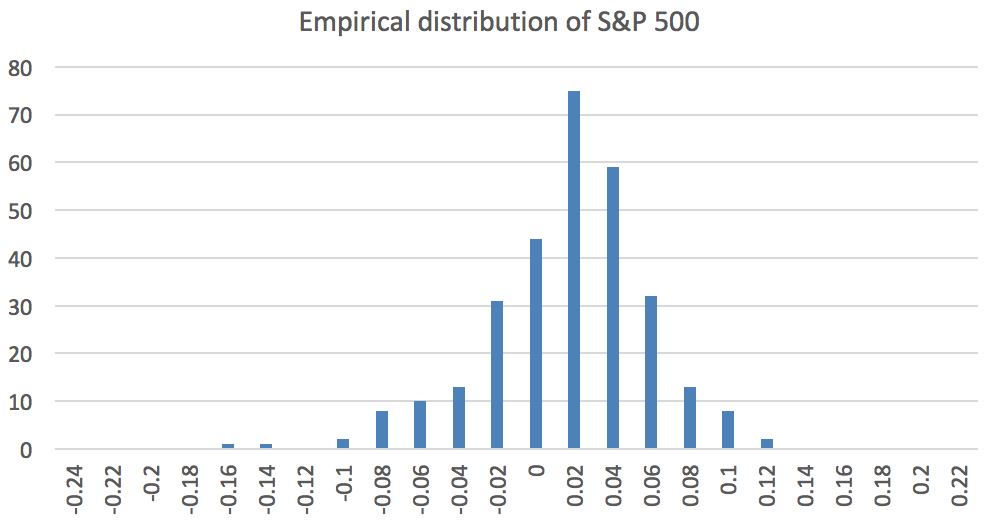
\includegraphics[width=300px]{./pic/hist.png}
\end{center}

\begin{center}
	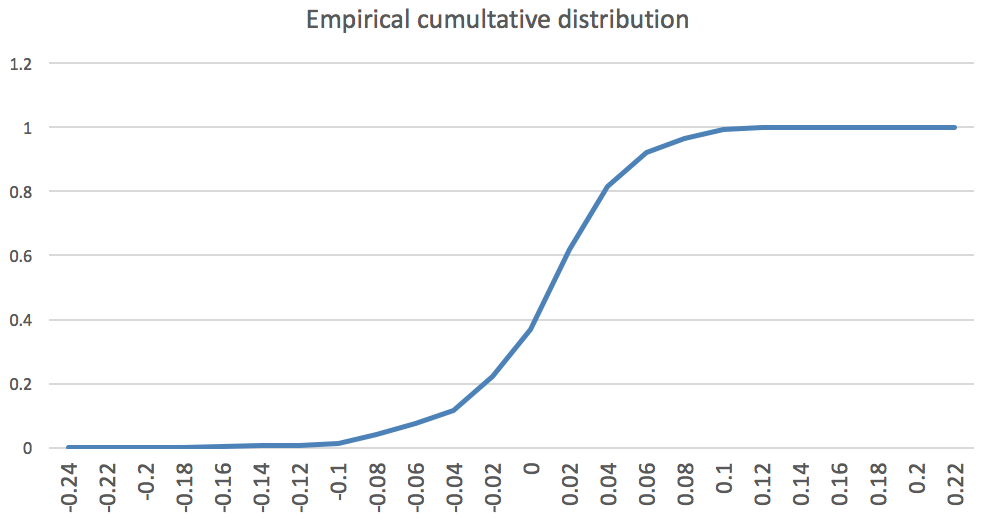
\includegraphics[width=300px]{./pic/distr.PNG}
\end{center}

\begin{center}
	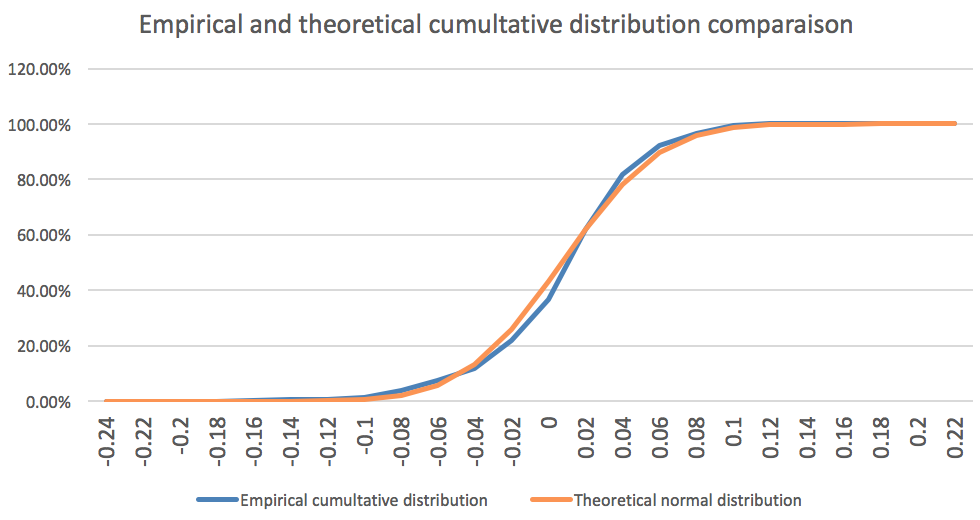
\includegraphics[width=300px]{./pic/distr_th.PNG}
\end{center}

In this last graph, we see that both the theoretical and the empirical distribution are about the same. This means that the return rate is almost described as a normal distribution.


%======= TABLEAU ===========
%\begin{center} %---------------Tab--------------
%\begin{tabular} {| c | c | c | c | c | c |}
%\hline
 %& & & & & $\\ \hline
%\end{tabular}
%\end{center}


%===========GRAPH================
%\begin{figure} %---------------------Graph---------------------------
%\begin{center}
%\includegraphics[width=12cm]{graph/ampli2} 
%\end{center}
%\caption{\em  \label{label}
%L�gende
%}
%\end{figure}


%========SUBGRAPH=======
%\begin{figure} [h] %----------- SubGraph ---------------------
%\centerline{
%\subfigure[ sublegend ] {\label{sfig:thetat} \includegraphics[width=7cm]{ graph/graph_convdt3 } }
%\subfigure[ sublegend ] {\label{sfig:thetafin} \includegraphics[width=7cm]{ graph/graph_convtfin } } 
%}
%\caption{\label{ label } 
%L�gende
%} 
%\end{figure}








\end{document} %%%% THE END %%%%
